\chapter{TINJAUAN PUSTAKA}

% Ubah konten-konten berikut sesuai dengan isi dari tinjauan pustaka
\section{Hasil penelitian/perancangan terdahulu}
Dari hasil kajian terhadap dua penelitian sebelumnya, terdapat beberapa poin penting yang menjadi acuan dan evaluasi untuk pengembangan alat dalam penelitian ini

\begin{enumerate}
    \item Hasil Penelitian Samuel Manallang (2020)
    
    Hasil penelitian Samuel Manallang (2020) yang berjudul \textit{Robot Pengisi Nomor Token Listrik} ini mengembangkan sistem pengisian token listrik yang memanfaatkan 12 solenoid sebagai penggerak untuk menekan tombol pada meteran listrik. Meskipun sistem tersebut berhasil dalam pengisian token secara otomatis, alat yang dikembangkan memiliki beberapa kelemahan, terutama dari segi ukuran dan kompleksitas. Ukuran alat yang besar serta penggunaan banyak solenoid membuat alat ini tidak praktis untuk digunakan di rumah-rumah atau skala komersial yang membutuhkan solusi yang lebih kompak dan efisien. Selain itu, sistem ini memerlukan daya yang cukup besar untuk menggerakkan banyak solenoid secara bersamaan, sehingga tidak efisien dari segi konsumsi energi. Oleh karena itu, alat tersebut kurang layak untuk diadopsi secara komersial maupun di rumah tangga umum. \parencite{manullang}

    \item Hasil Penelitian Danny Kurnianto, Aldi Wijaya, dan Muntaqo Alfin Amanaf (2022)

    Hasil penelitian yang berjudul \textit{Sistem Pengisian Token Listrik Jarak Jauh Berbasis IoT pada Alat Ukur Listrik Rumah} ini menggunakan meteran listrik khusus yang sudah dimodifikasi untuk memudahkan pengisian token secara otomatis. Meskipun alat ini lebih sederhana dan tidak memerlukan banyak komponen tambahan seperti solenoid, keterbatasan utama dari penelitian ini adalah ketergantungannya pada meteran listrik yang telah diubah. Modifikasi ini membuat alat tersebut sulit untuk diimplementasikan secara luas, terutama bagi pengguna listrik prabayar yang menggunakan meteran standar dari perusahaan penyedia listrik. Bagi masyarakat awam, menggunakan alat ini akan memerlukan penggantian meteran atau modifikasi yang tidak mudah dilakukan, sehingga mengurangi potensi adopsi alat ini di pasar. \parencite{kurnianto}
\end{enumerate}

\section{Teori/Konsep Dasar}

\subsection{Internet of Things}

% Contoh penggunaan referensi dari pustaka
\textit{Internet of Things} menjelaskan mengenai \textit{Things} atau barang yang memiliki akses internet dengan identitias nya masing - masing (\textit{UID} dan Alamat \textit{IP}) yang dapat melakukan perpindahan data antarlokasi, baik jarak dekat maupun jauh. Alat \textit{IoT} dapat terhubung ke Internet melalui kabel maupun nirkabel (\textit{Wi-Fi, NFC,} dll). Selagi terhubung dengan Internet maka objek itu masuk ke dalam kategori \textit{Internet of Things}, baik itu komputer, bola lampu, kunci pintu, dll. 

\textit{Internet of Things} merupakan sebuah konsep yang sangat esensial di zaman modern ini, karena dapat menghubungkan antara benda fisik dan benda digital yang memudahkan penggunanya untuk berkomunikasi dengan sebuah produk digital dan juga sebaliknya, sehingga terbentuklah sebuah integrasi antara kedua dunia yang sangat intuitif. Saat ini \textit{Internet of Things} menjadi salah satu faktor terjadinya revolusi di industri, yang disebut sebagai \textit{Industry 4.0} sesuai pada gambar \ref{fig:industry40}, yang mengedepankan inovasi menggunakan teknologi modern sebagai wahana untuk memanufaktur dan memproduksi dengan cara yang lebih efektif dan pintar. 

\begin{figure}[H]
    \centering
    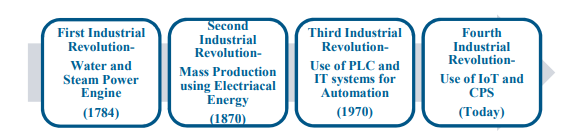
\includegraphics[width=0.8\linewidth]{gambar/industry-40.png}
    \caption{Evolusi industri dunia \cite{industry40}}
    \label{fig:industry40}
\end{figure}

Data adalah output utama dalam implementasi \textit{IoT}. Dimana fungsi \textit{IoT} sebenarnya, dengan bantuan sensor dan konektivitas, adalah untuk mencari informasi melalui data yang didapatkan. Dimana data menjadi alasan terbentuknya informasi yang sempurna jika data tersebut dapat dimanfaatkan dengan baik. Informasi sempurna inilah yang menjadi dasar pentingnya \textit{IoT} pada dunia teknologi, informasi memungkinkan kita untuk mengambil keputusan dan mengatur berdasarkan informasi yang konkrit, sehingga dapat digunakan sebagai acuan untuk melakukan automasi dalam berbagai aspek untuk kehidupan yang lebih efisien. \parencite{iot-sg}

Pada dasarnya arsitektur \textit{IoT} dibagi menjadi 3 bagian, yaitu lapisan \textit{Application, Network, dan Perception} dimana \textit{Application} atau aplikasi menjadi lapisan yang menyajikan data kepada pengguna juga berfungsi sebegai antarmuka dengan sistem IoT, \textit{Network} atau lapisan jaringan menghubunkan perangkat IoT dengan jaringan internet sehingga dapat berkomunikasi dengan perangkat lainnya, dan terakhir adalah \textit{Perception} atau lapisan persepsi bertugas untuk mengumpulkan data dari lingkungan tertentu dengan perangkat fisik melalui sensor dan aktuator.

Namun pada penulisan baru dilakukan abstraksi pada arsitektur dasar dari \textit{IoT} menjadi lima lapisan, lapisan tersebut dibagi menjadi \textit{Business, Application, Service Management, Object Abstraction, dan Objects}. \textit{Objects} atau lapisan objek sama seperti lapisan persepsi yang berfungsi untuk mengambil dan memproses data melalui sensor fisik, kemudian data yang telah diproses dikirim ke lapisan \textit{Object Abstraction} atau lapisan abstraksi objek yang bertugas untuk mengirim data ke lapisan \textit{Service Management} dengan berbagai protokol yang telah ditentukan di awal, baik itu RFID, 3G, \textit{WiFi, Bluetooth},dll. Kemudian lapisan \textit{Service Management} atau manajemen servis menghubungkan servis dengan pihak yang menggunakannya dengan menyamakan nama dan alamat sehingga dapat saling berkomunikasi dengan protokol jaringan. \textit{Application} atau lapisan aplikasi menyediakan servis pada sistem \textit{IoT} pada penggunanya dalam bentuk antarmuka dengan cara yang intuitif sehingga dapat dimengerti dengan mudah oleh manusia. Terakhir adalah lapisan \textit{Business} atau lapisan bisnis, yang mengatur secara keseluruhan sistem \textit{IoT} mulai dari aktivitas dan servis yang disediakan. Lapisan ini juga bertanggungjawab untuk membuat model bisnis, grafik, \textit{flowchart}, dll. sehingga memudahkan analisa dan pengembangan dari sistem \textit{IoT} yang digunakan. \parencite{iot-arab}

\subsection{Mikrokontroler ESP32}
ESP32 adalah sebuah mikrokontroler \textit{System on Chip (SOC)} oleh Espressif yang terintegrasi dengan \textit{Wi-Fi} dan \textit{Bluetooth}. ESP32 menggunakan prosesor 40nm Xtensa 32-bit dengan frekuensi 240Mhz, \textit{RAM} sebesar 520KB, dan \textit{ROM} sebesar 448KB. Prosesor yang digunakan ESP32 sangat rendah daya sehingga dapat digunakan dalam proyek dengan ukuran jejak yang kecil yang menggunakan baterai. Kapabilitas Wi-Fi dan Bluetooth dari ESP32 juga memudahkan penggunanya untuk  mengembangkan sistem yang dapat berkomunikasi secara nirkabel. Dalam ranah IoT, ESP32 termasuk ke dalam lapisan objek atau persepsi, dimana ESP32 dapat digunakan sebagai alat fisik yang mengumpulkan data dengan bantuan sensor yang dapat dihubungkan melalui 30 \textit{GPIO (General Purpose Input/Output)} yang ada pada ESP32. Aplikasi dari ESP32 tidak terbatas, dimana dapat diimplementasikan ekdalam sistem otomasi, \textit{Wearable Devices}, sistem sensor jaringan, robotika, dan banyak lagi. \parencite{esp32}

Berikut adalah pin yang tersedia pada ESP32 SoC,

\begin{figure}[H]
    \centering
    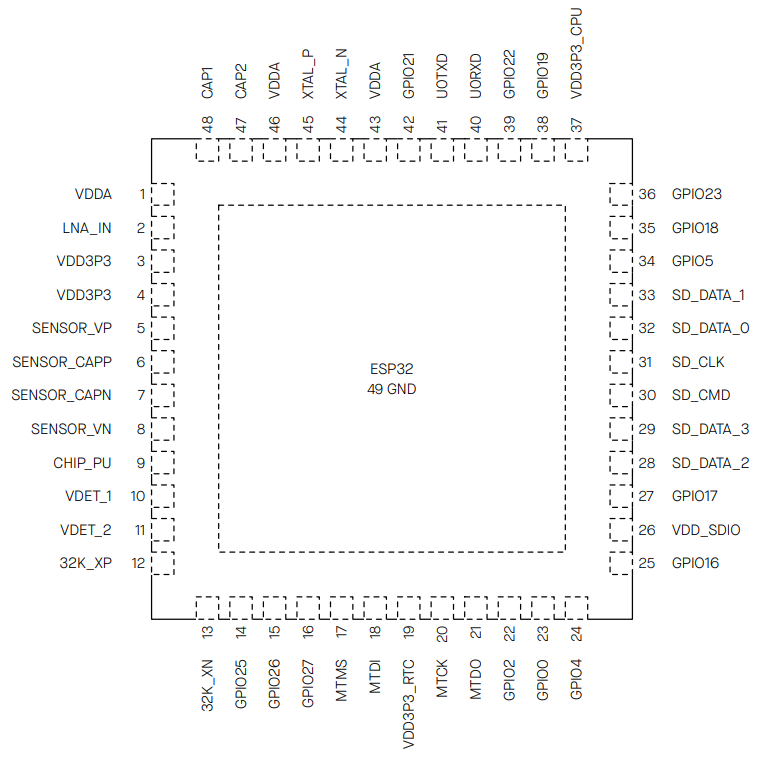
\includegraphics[width=0.45\linewidth]{gambar/pinout-esp32.png}
    \caption{\emph{Pinout} dari SoC ESP32}
    \label{fig:esp-32-pinout}
\end{figure}

Fungsi dari tiap pin bisa lebih dari satu, power pin yang ada pada ESP32 adalah sebagai berikut, dimana Vin adalah pin untuk memberikan daya dengan tegangan 5V - 12V, kemudian pin 3.3V yang digunakan untuk memberikan daya kepada perangkat eksternal, dan GND yang digunakan sebagai ground dari perangkat ESP32.
Ada 40 pin \textit{GPIO} pada ESP32 yang memiliki fungsi yang berbeda - beda. Pin GPIO 0-5 dan 12-33 memiliki fungsi digital input dan output dan pin 34-39 digunakan sebagai input saja, sedangkan pin 6-11 terhubung secara internal dalam ESP32. Beberapa dari pin ini juga memiliki fungsi lain seperti komunikasi UART, I2C, dan PWM juga beberapa pin yang digunakan sebagai \textit{Analog to Digital Converter dan Digital to Analog Converter}. Fungsi - fungsi yang lengkap ini sangat membantu dalam pembuatan proyek yang bervariasi.

Beberapa modul koneksi nirkabel yang dapat diutilisasikan oleh ESP32 adalah Bluetooth dan Wi-Fi. Teknologi Bluetooth yang digunakan pada SoC ESP32 adalah versi 4.2 dengan \textit{bandwidth} maksimum hingga 4 Mbps dan power transmisi sebesar +9 dBm juga sudah dapat terhubung ke lebih dari satu perangkat. Wi-Fi yang terintegrasi dalam ESP32 menggunakan frekuensi di 2.4GHz dengan protokol 802.11b/g/n yang dapat melakukan transmisi data hingga 150 Mbps. Salah satu protokol yang dapat digunakan dengan Bluetooth dan Wi-Fi pada ESP32 adalah protokol ESP-NOW, dimana protokol tersebut memungkinkan komunikasi antara perangkat ESP32 menggunakan daya dan \textit{latency} yang rendah tanpa membutuhkan akses poin atau router. \parencite{esp32-datasheer}

\subsection{\textit{Computer Numerical Control}}
Mesin kontrol numerik adalah mesin yang diatur menggunakan perhitungan numerik untuk menjalankan suatu tujuan tertentu, mesin ini dibagi menjadi dua, yaitu mesin pemotong dan mesin non-pemotong. Mesing pemotong artinya mesing yang menghilangkan materi dari sebuah objek untuk menciptakan suatu bentuk tertentu, contoh dari mesin ini adalah mesin \textit{milling} dan mesin bubut. Sedangkan mesin non-pemotong merubah bentuk dari sebuah objek dengan memberikan gaya kepada objek, contohnya adalah mesin pres. Sistem gerak pada robot juga termasuk kedalam mesin non-pemotong. CNC atau \textit{Computer Numerical Control} adalah sistem atau mesin kontrol numerik yang diatur dengan bantuan perhitungan komputer sehingga dapat dikontrol dengan akurasi dan efisiensi. 

Mesin CNC merubah perhitungan dari sebuah sistem numerik dengan menggunakan me- kanisme penggerak yang digerakkan oleh servo, dimana merupakan sebuah motor yang bergerak pada sebuah \textit{axis} sesuai dengan perintah tertentu, namun pergerakan yang dilakukan oleh motor berbentuk pergerakan rotasi sehingga perlu diubah menjadi gerakan yang linear, ada beberapa cara yang dapat dilakukan untuk mengubah bentuk pergerakan tersebut, yang pertama adalah dengan menggunakan \textit{coupling} dan \textit{ball screw}, seperti pada gambar \ref{fig:nut-screw}, dimana sekrup akan berputar sesuai dengan perputaran motor dan mur yang terletak pada sekrup akan bergerak secara linier. Cara kedua adalah menggunakan sistem \textit{belt dan pulley}, seperti pada gambar \ref{fig:pulley}, yang mengubah pergerakan rotasi dari servo motor menjadi gerakan linier pada sabuk yang terpasang dalam sistem. 

\begin{figure}[H]
    \centering
    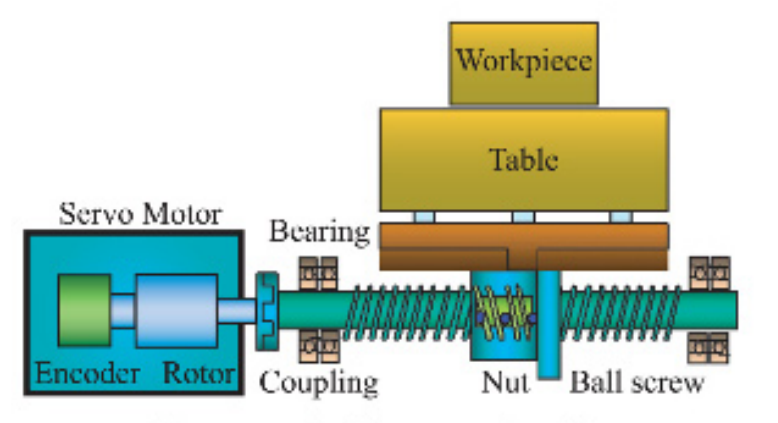
\includegraphics[width=0.5\linewidth]{gambar/nut-screw-mech.png}
    \caption{Sistem gerak linear dengan sekrup dan mur}
    \label{fig:nut-screw}
\end{figure}

\begin{figure}[H]
    \centering
    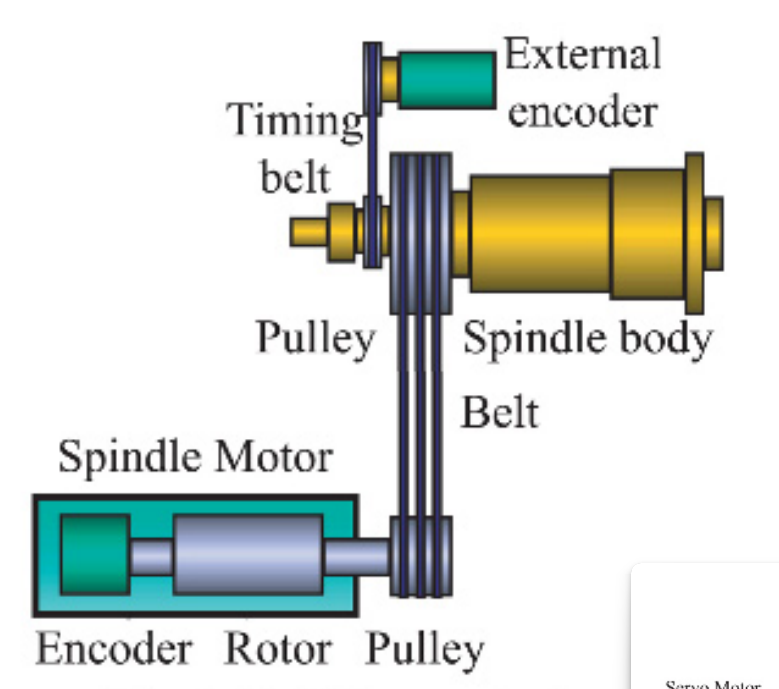
\includegraphics[width=0.4\linewidth]{gambar/pully-mech.png}
    \caption{Sistem gerak liner dengan sistem \textit{belt dan pulley}}
    \label{fig:pulley}
\end{figure}

Ada beberapa jenis yang dapat digunakan sebagai motor penggerak dalam sistem \textit{CNC}, yaitu servo motor DC, servo motor AC sinkronus, dan servo motor AC induksi, sesuai dengan gambar \ref{fig:servo-types}.

\begin{figure}[H]
    \centering
    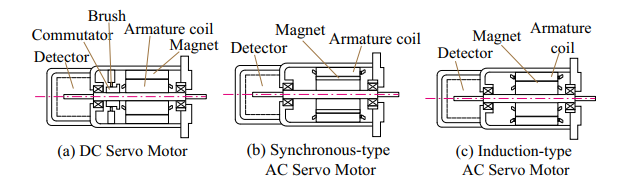
\includegraphics[width=0.8\linewidth]{gambar/servo-motor-diff.png}
    \caption{Tipe - tipe servo motor}
    \label{fig:servo-types}
\end{figure}

Servo motor DC, seperti pada gambar \ref{fig:servo-types}a, merupakan motor yang terbuat dari yang stator terdiri dari bingkai silinder, yang berperan sebagai jalur untuk fluks magnetik dan pendukung mekanis, dan magnet, yang dipasang ke bagian dalam bingkai. Rotor terdiri dari poros dan sikat. Komutator dan rangka penyangga logam rotor (inti rotor) dipasang pada bagian luar poros dan angker dililitkan pada rangka penyangga logam rotor. Sikat yang memasok arus melalui komutator dibuat dengan kumparan jangkar. Di bagian belakang poros, detektor untuk mendeteksi kecepatan rotasi terpasang pada rotor. Servo motor AC sinkronus merupakan servo yang tebuat dari stator yang terdiri dari rangka silinder dan inti stator. Inti stator terletak di dalam rangka dan kumparan jangkar dililitkan di sekitar inti stator. Ujung kumparan dihubungkan dengan kabel utama dan arus disediakan dari kabel utama. Rotor terdiri dari poros dan magnet permanen dan magnet permanen dipasang di bagian luar poros. Pada motor servo AC tipe sinkron, magnet dipasang ke rotor dan kumparan jangkar dililitkan di sekitar stator tidak seperti motor servo DC. Oleh karena itu, suplai arus dimungkinkan dari luar tanpa stator dan motor servo AC tipe sinkron disebut “motor servo \textit{brushless}” karena karakteristik struktural ini. Karena struktur ini memungkinkan untuk mendinginkan inti stator langsung dari luar, maka dimungkinkan untuk menahan peningkatan suhu. Terakhir ada motor servo AC induksi, dimana struktur motor servo AC tipe induksi identik dengan motor induksi pada umumnya. Jika arus bolak-balik multi-fase mengalir melalui kumparan stator, arus diinduksi dalam kumparan rotor dan arus induksi menghasilkan torsi. Pada motor servo AC jenis ini, stator terdiri dari rangka, inti stator, kumparan jangkar, dan kawat timah. Rotor terdiri dari poros dan inti rotor yang dibangun dengan konduktor.

Kemudian dalam sistem CNC juga terdapat enkoder, yaitu perangkat yang mendeteksi posisi saat ini untuk kontrol posisi, umumnya, dibangun di ujung poros transmisi daya. Untuk mengontrol kecepatan, kecepatan dideteksi oleh sensor atau dihitung oleh data kontrol posisi yang terdeteksi dari encoder. Metode untuk mendeteksi kecepatan menggunakan encoder, cara menghitung pulsa yang dihasilkan dalam satuan waktu dan sarana untuk mendeteksi interval antara pulsa bersama. Ada dua macam jenis enkoder, yaitu optikal dan magnetik. Bagian deteksi encoder tipe magnetik berbeda dengan encoder tipe optik, tetapi kedua jenis encoder ini menghasilkan sinyal output dengan cara yang sama.

Kemudian ada \textit{resolver dan speed sensor}, \textit{resolver} adalah detektor sudut dan posisi rotasi dan digunakan sebagai sensor motor. Tidak seperti encoder yang menghasilkan sinyal output dalam format digital, resolver menghasilkan output dalam format analog. \textit{Resolver} terdiri dari stator, rotor, dan trafo rotasi. Kumparan stator dan rotor disusun untuk membuat distribusi fluks magnetik menjadi gelombang sinus sehubungan dengan sudut. \textit{Resolver} memiliki struktur yang mirip dengan motor dan tidak peka terhadap getaran dan guncangan mekanis. Selain itu, karena outputnya adalah sinyal analog, maka transmisi sinyal jarak jauh dan miniaturisasi perangkat dimungkinkan. Namun demikian, sirkuit pemrosesan sinyal rumit dan perangkat ini lebih mahal daripada rotary encoder. Sedangkan \textit{speed sensor} sesuai namanya adalah sensor kecepatan dalam suatu sistem CNC.

Selain motor dan sensor, ada tiga komponen penting lainnya dalam sebuah sistem CNC yaitu \textit{Linear Movement Guide}, \textit{Coupling}, dan \textit{Control Loop}. \textit{Linear Movement Guide} merupakan sebuah kompenen fisik yang digunakan sebagai jalur untuk sistem CNC fungsi dari komponen ini adalah memastikan pergerakan dalam sistem tetap akurat dan baik. \textit{Linear Movement Guide} terdiri dari rel pemandu berbentuk M dan bagian pemindahan. \textit{Bearing} berada di antara rel pemandu dan bagian pemindahan dan pelumas disuplai ke permukaan rel\textit{Linear Movement Guide} untuk mengurangi gesekan saat bagian pemindahan bergerak. Berikut pada gambar \ref{fig:lmg} adalah contoh dari \textit{Linear Movement Guide}.

\begin{figure}[H]
    \centering
    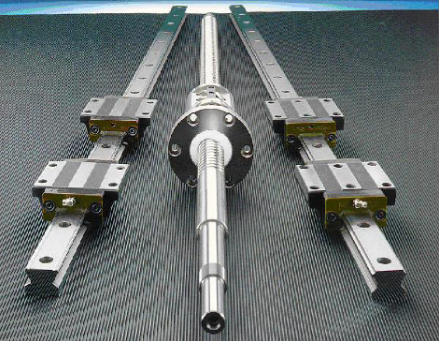
\includegraphics[width=0.6\linewidth]{gambar/lm-gudie.png}
    \caption{\textit{Linear Movement Guide}}
    \label{fig:lmg}
\end{figure}

\textit{Coupling} atau kopling merupakan merupakan salah satu komponen mesin CNC yang menghubungkan poros motor servo dengan sekrup bola. Ketika sekrup bola dan motor servo disambungkan, bagian tengah porosnya harus identik. Namun, dalam praktiknya, ini sangat sulit. Untuk alasan ini, kopling harus dirancang agar tidak sensitif terhadap pusat rotasi yang tidak sejajar. Dan \textit{Control Loop} merupakan rangakaian kontrol yang dilakukan terhadap mesin CNC, kontrol ini dilakukan secara kontinius sehingga pergerakan yang dilakukan oleh mesin CNC akurat. Kontrol ini dapat dilakukan dengan akurat dengan menggunakan sensor dan motor yang menjadi komponen utama dari CNC.

Sistem CNC dapat diatur dengan menggunakan instruksi yang diberikan secara program, instruksi ini dinamakan sebagai \textit{G-Code} yang disiapkan sebelum mesin CNC berfungsi. Kode ini berisi lintasan, kecepatan, dan posisi alat dalam koordinat X, Y, dan Z. Kontrol yang sudah terprogram tersebut akan dioperasikan kepada \textit{Driving Motor} dan sensor pada sistem \textit{CNC}. \parencite{cnc}

\subsection{\textit{Computer Assisted Design (CAD)}}

\textit{CAD} atau \textit{Computer Assited Design} adalah sistem yang digunakan untuk drafting, desain,
simulasi, analisis, dan manufaktur sebuah produk. CAD biasanya digunakan untuk proyek teknik. 
Sistem CAD memiliki beberapa aplikasi dalam penggunaanya, yang pertama dan utama yaitu \textbf{modul geometris} 
atau pemanfaatan representasi geometri yang tepat, di mana model dibuat menggunakan entitas dasar seperti 
titik, garis, kurva, dan bentuk 3D. salah satu konsep kunci dalam CAD adalah pemodelan parametrik, yang memungkinkan pengguna 
mendefinisikan dimensi sebagai parameter yang dapat dengan mudah diubah, sehingga desain dapat 
diperbarui secara otomatis tanpa harus menggambar ulang secara manual. Dengan pendekatan ini, 
perubahan dalam satu bagian desain secara otomatis memperbarui bagian lain yang terkait, menjaga 
konsistensi dan efisiensi. Kemudian ada \textbf{modul aplikasi} yaitu kemampuan sistem CAD untuk menghasilkan 
tidak hanya sebuah model, namun sebuah objek yang fungsional yang dapat direalisasikan ke dunia nyata
dengan bantuan alat eksternal, dan sistem tersebut harus dapat melakukan kalkulasi dan simulasi yang
akurat sehingga dapat menjadi visualisasi yang baik dari produk akhir. \textbf{Modul pemrograman} 
menyediakan kemampuan untuk melakukan pemrograman dengan bahasa pemrograman tertetntu
 terhadap produk yang dihasilkan sehingga desain 
dapat menyesuaikan hasil secara detail sesuai keinginan penggunanya. Terakhir adalah 
\textbf{modul komunikasi} dan \textbf{modul kolaborasi}, modul komunikasi sangat penting dalam 
proyek yang membutuhkan berbagai alat dalam pengerjaannya, baik itu secara perangkat keras maupun 
perangkat lunak, sebuah sistem CAD harus dapat berkomunikasi dengan alat lainnya agar tercipta
ekosistem desain dan manufaktur yang baik dan mudah dilakukan, sedangkan modul kolaborasi 
merupakan sesuatu yang berkembang sejak adanya internet, dimana sebuah desain dapat dikerjakan 
secara kolaboratif dengan bantuan internet. 

Beberapa contoh perangkat lunak Computer-Aided Design (CAD) yang banyak digunakan di berbagai industri
adalah AutoCAD, SolidWorks, dan Fusion 360, yang masing-masing memiliki keunggulan dan perbedaan 
khusus dalam fitur dan aplikasi yang ditawarkan. AutoCAD, yang dikembangkan oleh Autodesk, merupakan 
salah satu perangkat lunak CAD paling populer yang dikenal karena fleksibilitasnya dalam pembuatan 
gambar 2D dan model 3D. Perangkat lunak ini sering digunakan di bidang arsitektur, konstruksi, dan 
teknik sipil untuk merancang rencana struktur dan infrastruktur yang membutuhkan presisi tinggi, 
dengan antarmuka yang dirancang untuk memudahkan proses penggambaran teknis. Di sisi lain, 
SolidWorks adalah perangkat lunak CAD berbasis parametrik yang banyak digunakan dalam teknik 
mesin dan desain produk, terutama untuk perancangan komponen mekanik yang kompleks. 
SolidWorks menonjol dalam simulasi dan analisis desain, seperti analisis tegangan, dinamika fluida, 
dan optimasi desain, yang memungkinkan insinyur menguji kinerja model sebelum diproduksi. 
Perangkat lunak ini juga mendukung perakitan produk yang rumit dengan fitur-fitur seperti perakitan 
bergerak dan analisis beban, yang sangat berguna dalam pengembangan produk mekanis. Sementara itu, 
Fusion 360, yang juga merupakan produk Autodesk, menawarkan pendekatan inovatif dengan platform 
berbasis cloud yang memungkinkan kolaborasi real-time dan pengintegrasian fitur-fitur untuk 
pemodelan parametrik, simulasi, dan manufaktur aditif. Fusion 360 cocok untuk perancangan produk 
dan pembuatan prototipe karena menggabungkan desain, simulasi, dan proses manufaktur dalam satu 
antarmuka yang efisien. Perbedaan utama antara perangkat lunak ini terletak pada fokus penggunaannya: 
AutoCAD lebih fleksibel untuk berbagai jenis desain umum dan lebih banyak digunakan dalam bidang 
konstruksi, SolidWorks unggul dalam simulasi dan desain mekanik yang memerlukan analisis kinerja, 
sementara Fusion 360 menawarkan kemudahan kolaborasi berbasis cloud dan integrasi manufaktur yang 
ideal untuk proses pengembangan produk yang cepat dan kolaboratif. \parencite{masteringcad}

\subsection{Manufaktur Aditif (\textit{3D Printing})}
Manufaktur aditif adalah istilah formal untuk apa yang sering disebut sebagai pembuatan \textit{Rapid Prototyping} dan \textit{3D Printing}. \textit{Rapid Prototyping (RP)} adalah proses untuk membuat representasi sistem atau bagian dengan cepat sebelum dirilis atau dikomersialkan. Dengan kata lain, penekanannya adalah menciptakan sesuatu dengan cepat, di mana hasilnya adalah prototipe atau model dasar yang nantinya akan menjadi model lanjutan dan, pada akhirnya, menjadi produk yang siap dipasarkan. Konsep manufaktur aditif ini direalisasikan melalui proses \textit{layering}, di mana pembuatan komponen melibatkan penggunaan lapisan-lapisan 2-dimensi yang diperoleh dari perpotongan model 3D, yang kemudian ditumpuk secara berurutan untuk membentuk struktur akhir. Hampir semua teknologi manufaktur aditif mengikuti prinsip ini, yaitu membuat komponen dengan menambahkan material lapis demi lapis secara presisi. Lapisan-lapisan ini dapat bervariasi dalam ketebalan, tergantung pada teknologi yang digunakan. Dengan pendekatan manufaktur berbasis lapisan ini, proses pembuatan prototipe dapat dipercepat dan biaya pengembangan dapat dikurangi, sehingga sangat bermanfaat dalam inovasi produk dan pengembangan iteratif.

Aplikasi dari manufaktur aditif telah berkembang pesat dalam beberapa tahun terakhir, terutama karena kemampuan teknologi ini untuk menciptakan visualisasi produk yang sedang dikembangkan dengan lebih efektif dan intuitif. Model fisik yang dihasilkan oleh manufaktur aditif menawarkan keuntungan yang signifikan dibandingkan dengan gambaran 2-dimensi atau \textit{rendering} 3-dimensi yang biasa digunakan dalam proses desain. Keunggulan utama dari model fisik adalah kemudahan dalam pemahaman oleh penggunanya, yang dapat mempelajari dan mengevaluasi bentuk dan fitur produk dengan lebih akurat. 
Peningkatan yang konsisten dalam kualitas manufaktur aditif, yang mencakup akurasi geometrik, keanekaragaman material, dan kecepatan produksi, telah memungkinkan teknologi ini digunakan dalam berbagai pengujian yang lebih kritis. Produk yang dihasilkan kini dapat dievaluasi berdasarkan tiga kriteria utama, yaitu \textit{Form, Fit, dan Function}. \textit{Form} mengacu pada kriteria yang memastikan bahwa model fisik yang dihasilkan benar-benar sesuai dengan bentuk estetika dan fungsi dasar dari produk yang direncanakan. Kriteria ini sangat penting untuk menentukan apakah produk secara visual dan fisik memenuhi harapan awal yang diinginkan.
Selanjutnya, ada kriteria \textit{Fit}, yang berfokus pada akurasi dimensi dan toleransi dari komponen yang diproduksi. Komponen ini harus sesuai dengan spesifikasi desain untuk memastikan bahwa mereka dapat dirakit dengan sempurna ke dalam sistem yang lebih besar tanpa adanya celah atau masalah lain yang dapat mempengaruhi kinerja produk. Uji \textit{Fit} sering kali mencakup pengukuran presisi yang sangat ketat, karena kesalahan kecil dalam dimensi dapat menyebabkan masalah dalam perakitan.
Kriteria terakhir adalah \textit{Function}, yang menguji apakah produk atau komponen yang dihasilkan memiliki material dan karakteristik fungsional yang sesuai dengan tujuan akhir desain. Aspek ini memastikan bahwa produk dapat bertahan dalam kondisi lingkungan nyata, seperti tekanan, suhu, atau gaya mekanis, yang mungkin dihadapi selama penggunaannya. Pengujian \textit{Function} sering kali mencakup simulasi kondisi dunia nyata untuk memverifikasi bahwa performa produk tidak hanya sesuai secara fisik tetapi juga secara operasional, menjadikan manufaktur aditif alat yang sangat fungsional dalam proses iteratif pengembangan produk.

Prinsip dasar dari teknologi ini adalah bahwa sebuah model, yang awalnya dibuat dengan menggunakan sistem \textit{Computer-Aided Design} (CAD) tiga dimensi, dapat difabrikasi secara langsung tanpa memerlukan perencanaan proses. Meskipun pada kenyataannya tidak sesederhana kedengarannya, teknologi manufaktur aditif tentu saja secara signifikan menyederhanakan proses produksi objek 3D yang kompleks secara langsung dari data CAD. Proses manufaktur lainnya memerlukan analisis yang cermat dan terperinci dari geometri bagian untuk menentukan hal-hal seperti urutan fitur yang berbeda yang dapat dibuat, alat dan proses apa yang harus digunakan, dan perlengkapan tambahan apa yang mungkin diperlukan untuk menyelesaikan bagian tersebut. Sebaliknya, manufaktur aditif hanya membutuhkan beberapa detail dimensi dasar dan sedikit pemahaman tentang cara kerja mesin manufaktur aditif dan bahan yang digunakan untuk membuat komponen. Kunci dari cara kerja manufaktur aditif adalah bahwa komponen dibuat dengan menambahkan material secara berlapis-lapis; setiap lapisan merupakan penampang tipis dari komponen yang berasal dari data CAD asli. Tentunya dalam dunia fisik, setiap lapisan harus memiliki ketebalan yang terbatas sehingga bagian yang dihasilkan akan menjadi perkiraan dari data asli, seperti yang diilustrasikan oleh gambar \ref{fig:cad}. Semakin tipis setiap lapisan, semakin dekat bagian akhir dengan aslinya. Semua mesin manufaktur aditif yang dikomersialkan hingga saat ini menggunakan pendekatan berbasis lapisan, dan perbedaan utamanya terletak pada bahan yang dapat digunakan, bagaimana lapisan dibuat, dan bagaimana lapisan diikat satu sama lain. Perbedaan tersebut akan menentukan faktor-faktor seperti keakuratan bagian akhir serta sifat material dan sifat mekanisnya. Perbedaan tersebut juga akan menentukan faktor-faktor seperti seberapa cepat komponen dapat dibuat, berapa banyak pasca-pemrosesan yang diperlukan, ukuran mesin manufaktur aditif yang digunakan, dan biaya keseluruhan mesin dan proses.

\begin{figure}[H]
    \centering
    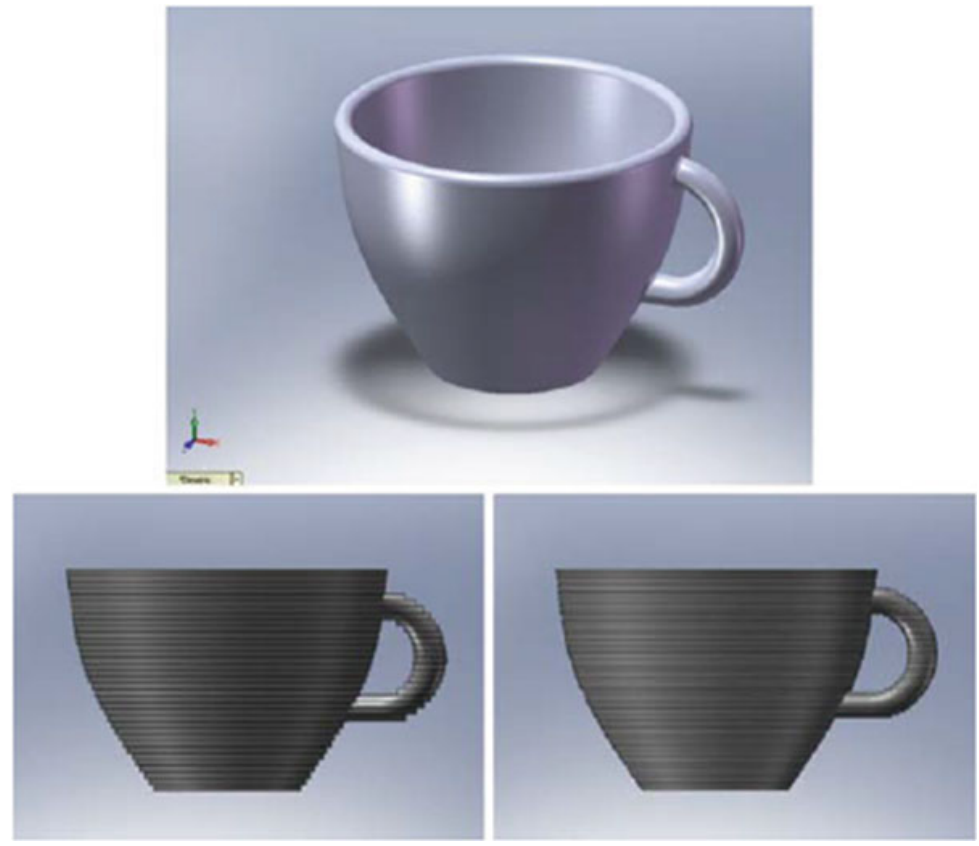
\includegraphics[width=0.6\linewidth]{gambar/cad-image.png}
    \caption{Rendering tiga dimensi dengan menggunakan \textit{Computer Aided Design}}
    \label{fig:cad}
\end{figure}

Seperti yang sudah dijelaskan diatas, manufaktur aditif secara keseluruhan menggunakan pendekatan sama yaitu dengan berbasis lapisan, namun dapat diklasifikasikan sesuai dengan teknologi yang digunakan untuk menghasilkan tiap lapisan tersebut. Jenis dari manufaktur aditif sangat banyak, namun pada umunya yang sering digunakan adalah \textit{SLA, SLS, dan FDM}. \textit{SLA atau Stereolithography} atau yang disebut juga sebagai \textit{Vat Photpolymerisation} adalah salah satu bentuk dari manufaktur aditif yang memanfaatkan sinar laser ultraviolet yang dapat menyebabkan material tertentu (seperti resin) berubah menjadi sebuah polymer yang mengeras sehingga menghasilkan sebuah objek 3-dimensi. \textit{SLS} atau \textit{Selective Laser Sintering} juga sebuah teknik manufaktur aditif yang menggunakan laser, namun laser yang digunakan merupakan laser dengan suhu tinggi yang dapat menyebabkan material tertentu (nilon atau polyamida) yang awalnya berbentuk bubuk, saling mengikat satu sama lain karna suhu tinggi tersebut sehingga dapat mengeras yang dilakukan dari tiap lapisan - lapisan dengan tinggi tertentu dan menghasilkan sebuah objek. Terakhir adalah \textit{FDM} atau \textit{Fused Deposition Modelling} adalah teknik manufaktur aditif yang menggunakan bahan plastik yang dipanaskan pada suhu tertentu (sesuai dengan jenis plastik yang digunakan) untuk menghasilkan sebuah bentuk tertentu, kemudian berbagi bentuk - bentuk ini ditumpuk sehingga menghasilkan barang 3-dimensi.

Berikut adalah beberapa contoh dari alat - alat manufaktur aditif

\begin{figure}[H]
    \centering
    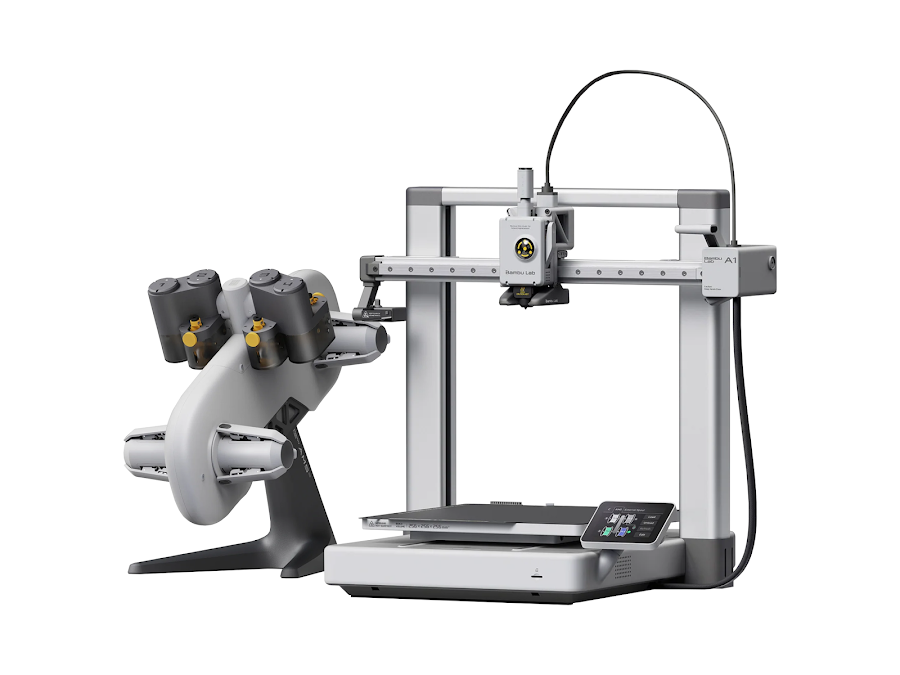
\includegraphics[width=0.35\linewidth]{gambar/fdm-3d-printer.png}
    \caption{Alat 3D Printer dengan Teknologi FDM \textit{(Fused Deposition Modelling)}}
    \label{fig:fdm-3d-printer}
\end{figure}

\begin{figure}[H]
    \centering
    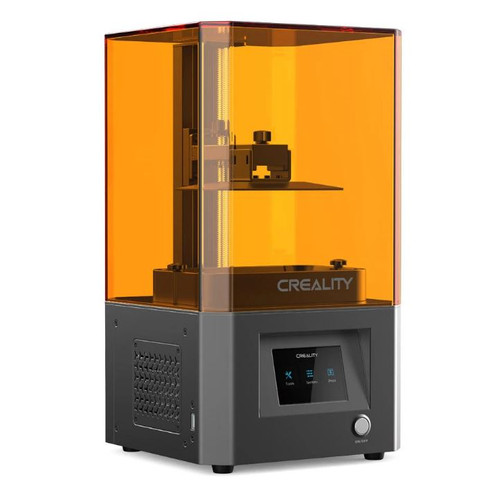
\includegraphics[width=0.25\linewidth]{gambar/sla-3d-printer.jpg}
    \caption{Alat 3D Printer dengan Teknologi SLA \textit{(Stereolithography)}}
    \label{fig:sla-3d-printer}
\end{figure}

\begin{figure}[H]
    \centering
    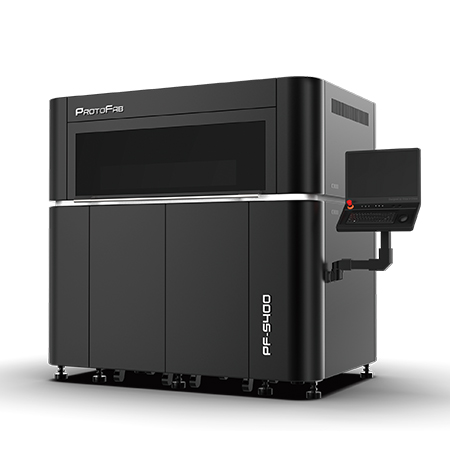
\includegraphics[width=0.3\linewidth]{gambar/sls-3d-printer.jpg}
    \caption{Alat 3D Printer dengan Teknologi SLS \textit{(Selective Laser Sintering)}}
    \label{fig:sls-3d-printer}
\end{figure}

Secara luas manufaktur aditif memiliki banyak kesamaan dengan teknologi mesin CNC. Dimana merupakan sebuah alat yang menghasilkan produk menggunakan bantuan komputer. Perbedaan utama dari kedua teknik ini adalah teknik yang digunakan dimana alat CNC utamanya menggunakan teknik subtraktif yang membutuhkan sebuah blok material tertentu untuk menghasilkan sebuah produk dengan desain yang telah ditentukan. Namun ada beberapa hal lainnya yang lebih rinci yang dapat membedakan kedua teknik manufaktur ini, yaitu material, kecepatan, kompleksitas, akurasi, geometri, dan pemrograman. Secara material teknologi manufaktur aditif pada awalnya dikembangkan di sekitar bahan polimer, lilin, dan laminasi kertas. Selanjutnya, diperkenalkan bahan komposit, logam, dan keramik. Pemesinan CNC dapat digunakan untuk bahan lunak, seperti papan serat kepadatan menengah (MDF), busa yang dapat dikerjakan dengan mesin, lilin yang dapat dikerjakan dengan mesin, dan bahkan beberapa polimer. Secara kecepatan, Pemesinan CNC pada umumnya dapat membuang material jauh lebih cepat daripada mesin manufaktur aditif dapat menambahkan volume material yang sama. Namun, ini hanya sebagian dari gambaran, karena teknologi manufaktur aditif dapat digunakan untuk memproduksi komponen dalam satu tahap. Mesin CNC memerlukan penyiapan dan perencanaan proses yang cukup banyak, terutama karena komponen menjadi lebih kompleks dalam geometrinya. Secara kompleksitas, semakin tinggi kompleksitas geometris, semakin besar keunggulan teknik manufaktur aditif dibandingkan CNC. Jika CNC digunakan untuk membuat bagian secara langsung dalam satu bagian, maka mungkin ada beberapa fitur geometris yang tidak dapat dibuat. Karena alat pemesinan harus dibawa dalam spindel, mungkin ada kendala aksesibilitas atau benturan tertentu yang mencegah alat tersebut ditempatkan pada permukaan pemesinan suatu bagian. Proses AM tidak dibatasi dengan cara yang sama dan \textit{undercut} serta fitur internal dapat dengan mudah dibuat secara mudah tanpa perencanaan proses yang spesifik. Bagian-bagian tertentu tidak dapat dibuat dengan CNC kecuali jika dipecah menjadi beberapa komponen dan dipasang kembali pada tahap selanjutnya. Secara akurasi, mesin manufaktur aditif pada umumnya beroperasi dengan resolusi beberapa puluh mikron. Biasanya mesin AM juga memiliki resolusi yang berbeda di sepanjang sumbu ortogonal yang berbeda. Biasanya, sumbu build vertikal sesuai dengan ketebalan lapisan dan ini akan memiliki resolusi yang lebih rendah dibandingkan dengan dua sumbu pada \textit{build plate}.  Sedangkan akurasi pada mesin CNC, utamanya ditentukan oleh resolusi pemosisian yang serupa di sepanjang ketiga sumbu ortogonal dan oleh diameter alat potong putar. Ada beberapa faktor yang ditentukan oleh geometri pahat, seperti jari-jari sudut internal, tetapi ketebalan dinding bisa lebih tipis daripada diameter pahat karena ini adalah proses subtraktif. Dalam kedua kasus tersebut, detail yang sangat halus juga akan menjadi fungsi dari geometri dan sifat material yang diinginkan. Secara geometri, mesin manufaktur aditif pada dasarnya memecah masalah 3D yang rumit menjadi serangkaian penampang 2D sederhana dengan ketebalan nominal. Dengan cara ini, koneksi permukaan dalam 3D dihilangkan dan kontinuitas ditentukan oleh seberapa dekat kedekatan satu penampang dengan penampang yang berdekatan. Karena hal ini tidak dapat dengan mudah dilakukan dalam CNC, pemesinan permukaan biasanya harus dibuat dalam ruang 3D. Terakhir secara pemrograman, urutan pemgoraman untuk mesin CNC bisa sangat rumit, termasuk pemilihan pahat, pengaturan kecepatan mesin, posisi dan sudut pendekatan, dll. Banyak mesin manufaktur aditif juga memiliki opsi yang harus dipilih, tetapi kisaran, kerumitan, dan implikasi seputar pilihannya sangat minim jika dibandingkan. \parencite{3dprinting}

\newpage
\subsection{Meteran Listrik Prabayar}
Meteran Listrik Prabayar atau yang disebut sebagai Listrik Pintar, sesuai gambar \ref{fig:meteran-prabayar} merupakan alat yang dikeluarkan oleh PT. PLN dimana pembayaran listrik yang awalnya dilakukan diakhir pemakaian dan dihitung oleh PLN sekarang dilakukan dengan mengisi token secara prabayar sehingga pengguna bisa mengatur seberapa banyak listrik yang digunakan dengan lebih mudah.

\begin{figure}[H]
    \centering
    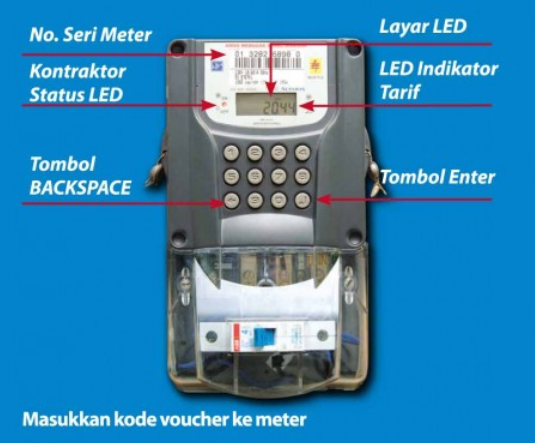
\includegraphics[width=0.5\linewidth]{gambar/meteran-prabayar.png}
    \caption{Meteran listrik prabayar PLN}
    \label{fig:meteran-prabayar}
\end{figure}

Mengisi token dapat dilakukan dengan cara membeli token melalui gerai ATM atau melalui loket pembayaran tagihan listrik online lainnya. Token atau pulsa listrik ini terdiri dari 20 digit angka yang dimasukkan kedalam kWh meteran khusus dari PLN. Token ini setelah dimasukkan akan berbentuk kWh yang dapat dilihat di meteran listrik dengan nilai yang telah ditentukan ketika membeli token.

Beberapa kelebihan yang dimiliki meteran listrik prabayar dibanding meteran tradisional ini adalah kemudahan untuk membeli token, monitoring dari meteran listrik yang lebih mudah, dan dapat privasi yang lebih terjaga. Dan jika energi listrik yang tersimpan di meteran sudah hampir habis, maka meteran akan memberikan sinyal awal suara agar segera dapat dilakukan pengisian ulang.